\chapter{Part III(a) - Memory Hierarchy - Virtual Memory - W.7.2}
\section{Segmentation Fault: Understanding the Cause}

Segmentation faults occur when a program attempts to access a memory location that is either invalid or restricted. Consider the following C code snippet:

\begin{center}
    \begin{tikzpicture}
        \node[rounded corners=30pt, draw=none] {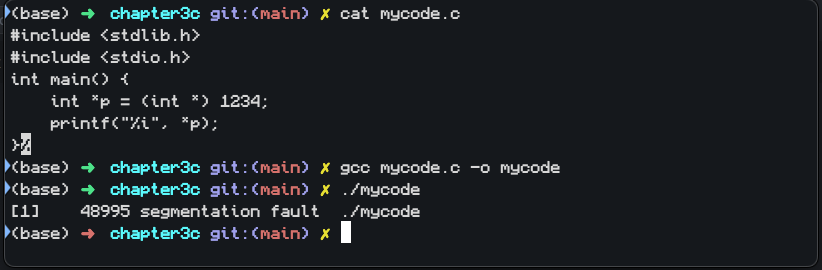
\includegraphics[width=0.65\textwidth]{chapters/chapter3c/images/terminal.png}};
    \end{tikzpicture}
\end{center}

In this example:
\begin{itemize}
    \item The pointer \texttt{p} is assigned the value \texttt{1234}, which is an arbitrary and invalid memory address.
    \item When the program attempts to dereference \texttt{p} using \texttt{*p} to access the value at memory address \texttt{1234}, it triggers a segmentation fault because the program does not have permission to access this memory.
\end{itemize}

\textbf{Why This Happens:}
\begin{itemize}
    \item Modern operating systems enforce memory protection, disallowing access to memory that the program does not explicitly allocate or own.
    \item Hardcoding arbitrary addresses, like \texttt{1234}, is unsafe and violates these protections.
\end{itemize}

\textbf{Assembly Analysis:}
The following assembly instructions illustrate how the invalid memory access occurs:
\begin{itemize}
    \item \texttt{li t0, 1234} -- Load the immediate value \texttt{1234} into register \texttt{t0}.
    \item \texttt{lw a1, 0(t0)} -- Attempt to load a word from address \texttt{1234}.
    \item This results in a segmentation fault because address \texttt{1234} is not valid or accessible.
\end{itemize}

We need to be able to protect memory and prevent such invalid accesses. This is where memory protection mechanisms come into play.

\subsection{Overview - Problems to Solve}
Three main problems need to be addressed:

\begin{enumerate}
    \item \textbf{Memory Protection:} How can we protect memory so that each program (or process) running simultaneously in the system can only access its own data? How can processes be isolated from each other?
    \item \textbf{Insufficient Main Memory:} What happens if the main memory (DRAM) is not sufficient for the execution of a program? Can we utilize the disk to address this limitation? If so, how?
    \item \textbf{Running Multiple Programs:} How can we run several programs (processes) simultaneously? How can multiple programs be loaded into memory efficiently, and where should they be stored?
\end{enumerate}
